\chapter{Schelling Segregation Model}\label{ch:2}

\resp{Bains, Arman Singh}

% \emph{
% Structure as\footnote{Remove this part from the report}:
% \begin{itemize}
% \item A short (max 1 page) explanation of the task, including references. Include mathematical concepts.
% \item Max 2 pages for the whole task (including figures)
% \item It is possible to use appendices for supplementary material, at the end of the report. Max 5 pages per task
% \end{itemize}
% A total of 3 pages + 5 supplementary pages per task
% }

% \section{A section...}
 
% Reference examples: book~\cite{barrat2008dynamical}, article~\cite{de2013mathematical}, website~\cite{weforumProtectingCritical}

\section{Introduction}

The stated goal of this project is to simulate a well known model of Sociophysics, possibly expanding on it through the lens of statistical mechanics and network theory. In particular, this paper focused on a segregation model developed first by Thomas C. Schelling \cite{schelling_dynamic_1971}, where individuals of two types on a network are allowed to move to vacant nodes to surround themselves with others of the same type, leading to de facto segregation. A second model, inspired by this, will also be discussed here, with the goal of showing that simulating the behavior of agents moving on top of the network is not necessary, rather it is sufficient to allow nodes to rewire some connections to expose that even a slight bias against dissimilar types will lead to segregation even in more abstract networks. In appendix \ref{ch:app2} Schelling's original model will be discussed again after simulating how various migration patterns might affect its dynamics. 

\section{Dynamics}

The one dimensional Schelling's model is implemented by employing a one dimensional lattice, with free boundary conditions. A fraction $r_0$ of the nodes will be labeled 0, representing vacancies, while the remaining nodes will be labeled $\pm1$, with $1$ representing agents of the majority type, $-1$ representing agents of the minority type and $m$ being the difference between the fraction of majority and minority agents. An individual is deemed to have utility 0 (i.e. unhappy) if more than half of his neighbors are of the opposite type (otherwise he will have utility 1). \\
The dynamics proceed by picking at random an unhappy agent, and checking if moving him in place of a random vacancy will increase its utility. As it can be seen in figure \ref{fig:schelling1DD}, displaying the mean total utility for the nodes of the minority type after 20 trials (as a function of the fraction of vacancies), a phase transition seems to occur. Indeed, a small number of vacancies may lead nodes of the minority type to be unhappy (because it would be unlikely for them to find a neighborhood with others of their type), whereas increasing vacancies will make it easier for them to relocate. It should be noted that the length of the lattice was initially set to $L=1,000$ to make the computations easier, but, as it can be seen from the plot, increasing $L$ to $10,000$ makes the curve smoother. That is because in $L=1,000$ there are too few vacancies, so it's quite hard for unhappy agents to find better nodes. Similarly, if the fraction of agents of the minority type is too little (i.e. $m$ is bigger), it's harder for them to find neighborhoods of similar agents where to relocate, increasing their total unhappiness. 
\begin{figure}[htbp]
    \centering
    \begin{minipage}[t]{0.48\linewidth}
        \centering
        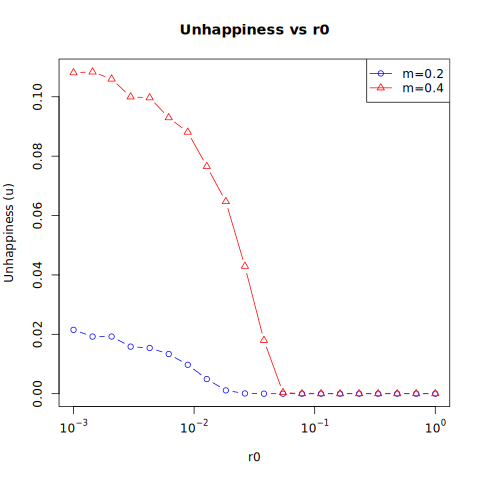
\includegraphics[width=\linewidth]{images/segregation_plot_1D.png}
        \caption{L=1,000.}
        \label{fig:1,000}
    \end{minipage}
    \hfill
    \begin{minipage}[t]{0.48\linewidth}
        \centering
        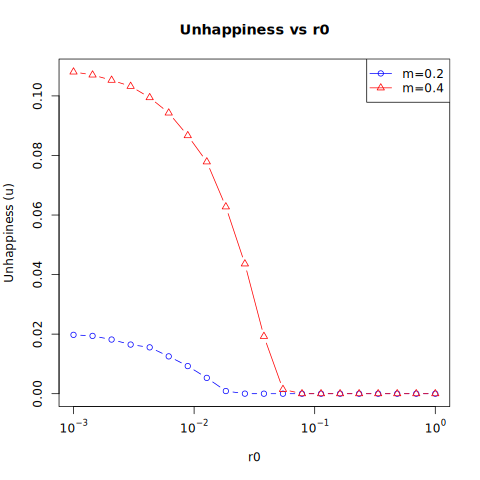
\includegraphics[width=\linewidth]{images/segregation_plot_1D_1e5.png}
        \caption{L=10,000}
        \label{fig:10,000}
    \end{minipage}
    \caption{}
    \label{fig:schelling1DD}
    
\end{figure}


\section{Abstract generalization}

In \cite{henry_emergence_2011}, it was shown that Schelling's initial proposal was unnecessarily restrictive if the goal was to prove that mild aversion to dissimilar types could result in segregation. Indeed, instead of simulating the dynamics of agents moving over a network, one could analyze the dynamics of the network itself, allowing its nodes to rewire themselves with a small probability. Therefore, what has been done for this project is to run several simulations where each node has been assigned to one of two types (with $70\%/ 30\%$ ratios), with the subsequent dynamics consists of picking an edge at random connecting dissimilar nodes, than allowing one to rewire such edge to another of similar type. Figure \ref{fig:henry_four} shows the homophily (i.e. the fractions of edges connecting nodes of the same type) and minority stress (i.e. the average fraction of dissimilar neighbors across all nodes of minority type), for networks of 400 nodes. The networks proposed have the same structure as those cited in chapter \ref{ch:1}, with the exception of the Erdős–Rényi network which was implemented with probability of edge drawing of 0.02.

% \begin{figure}[ht]
%     \centering
%     \begin{subfigure}[t]{0.2\textwidth}
%         \centering
%         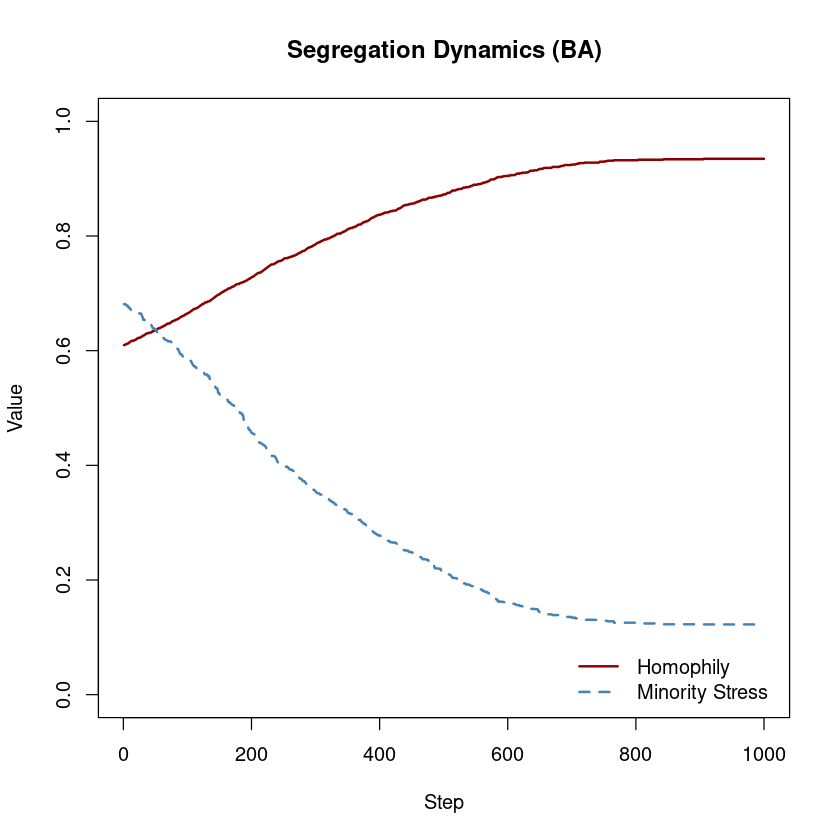
\includegraphics[width=\linewidth]{images/henryba.png}
%         \caption{Caption 1}
%     \end{subfigure}
%     \hfill
%     \begin{subfigure}[t]{0.2\textwidth}
%         \centering
%         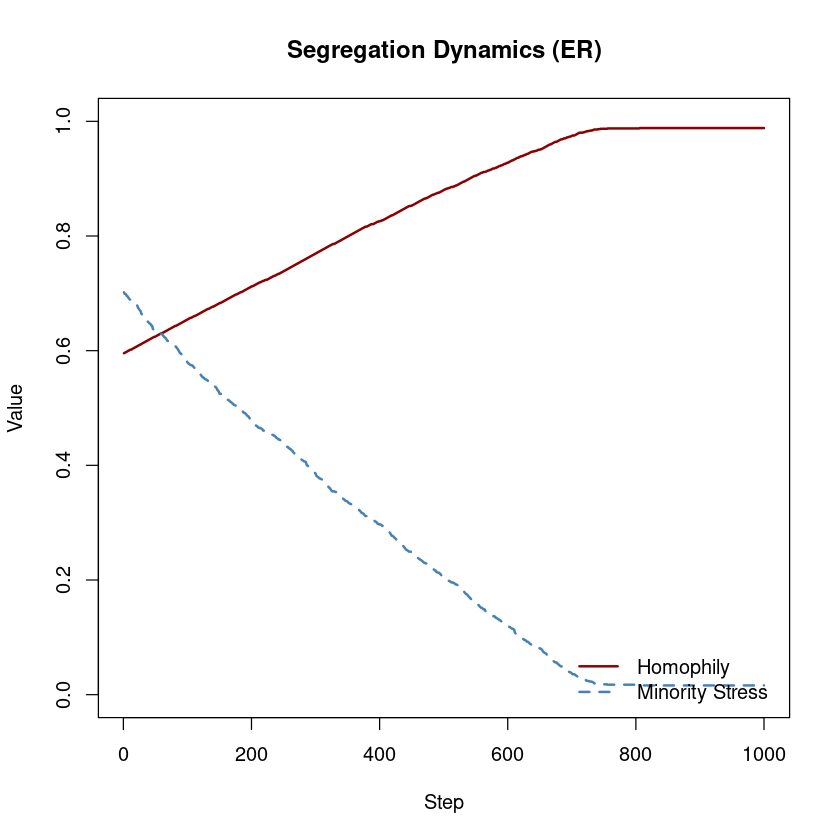
\includegraphics[width=\linewidth]{images/henryer.png}
%         \caption{Caption 2}
%     \end{subfigure}
%     \hfill
%     \begin{subfigure}[t]{0.2\textwidth}
%         \centering
%         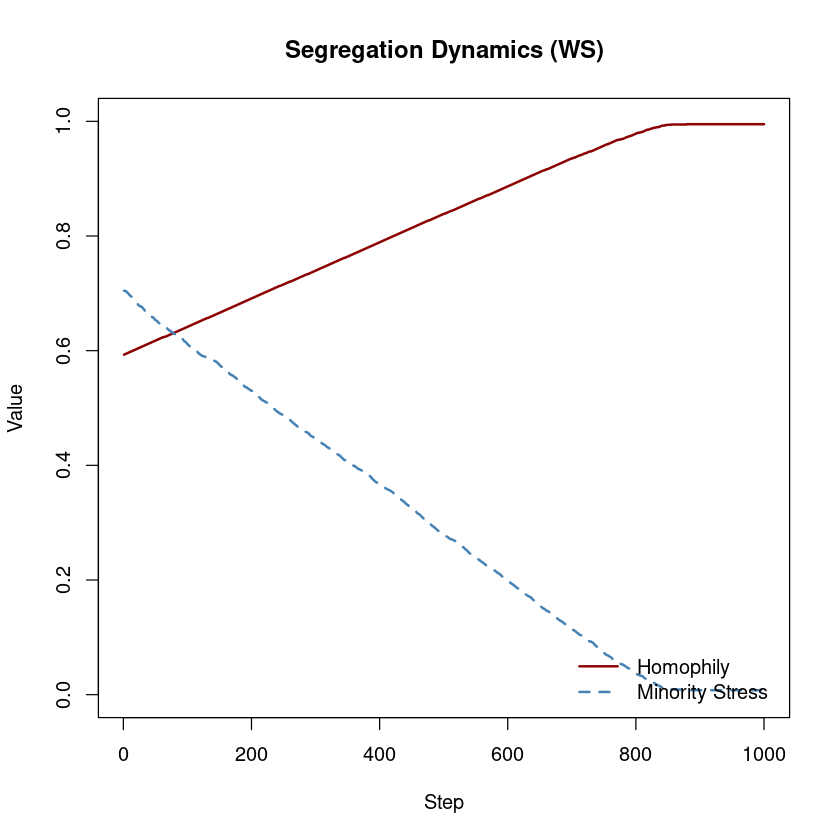
\includegraphics[width=\linewidth]{images/henryws.png}
%         \caption{Caption 3}
%     \end{subfigure}
%     \hfill
%     \begin{subfigure}[t]{0.2\textwidth}
%         \centering
%         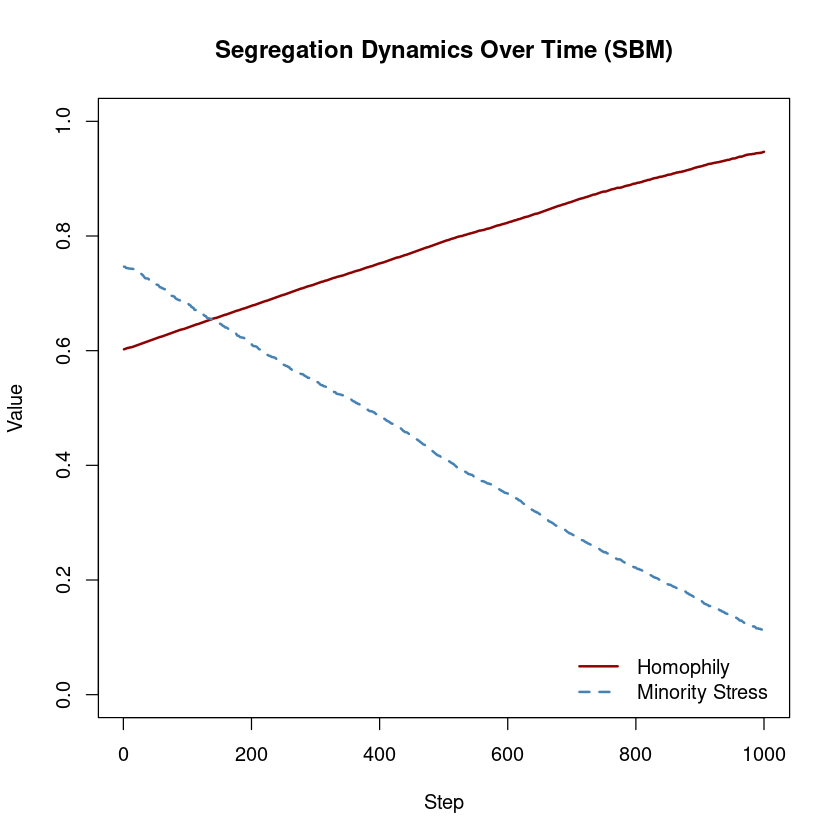
\includegraphics[width=\linewidth]{images/henrysbm.png}
%         \caption{Caption 4}
%     \end{subfigure}
%     \caption{Overall figure caption}
%     \label{fig:henry}
% \end{figure}




\begin{figure}[htbp]
    \centering
    \begin{minipage}[t]{0.24\linewidth}
        \centering
        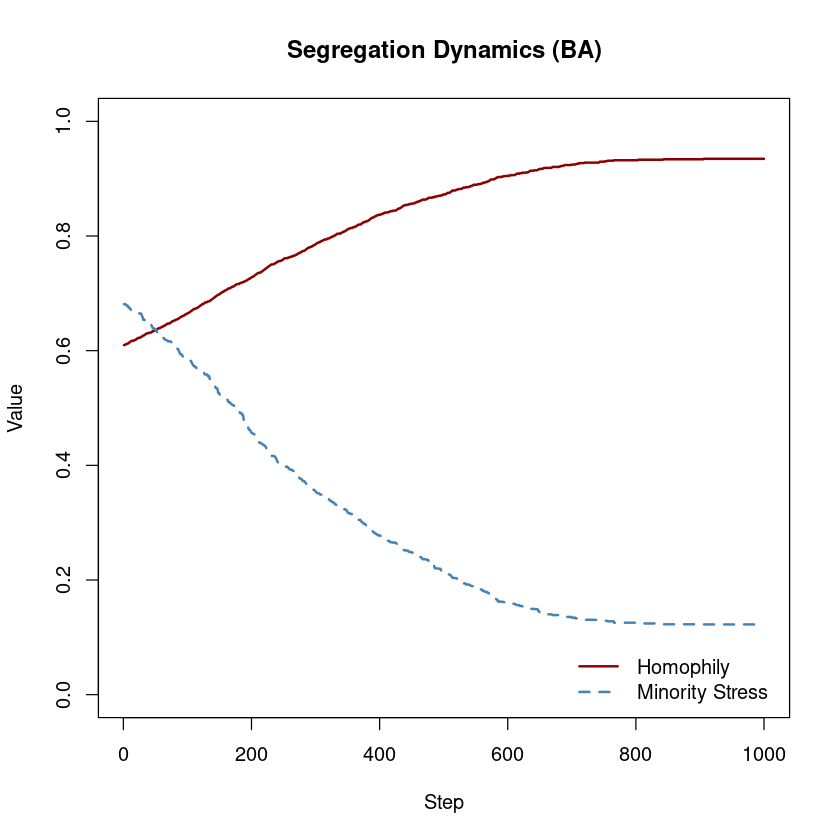
\includegraphics[width=\linewidth]{images/henryba.png}
        \caption{Barabási–Albert}
        \label{fig:henryba}
    \end{minipage}
    \hfill
    \begin{minipage}[t]{0.24\linewidth}
        \centering
        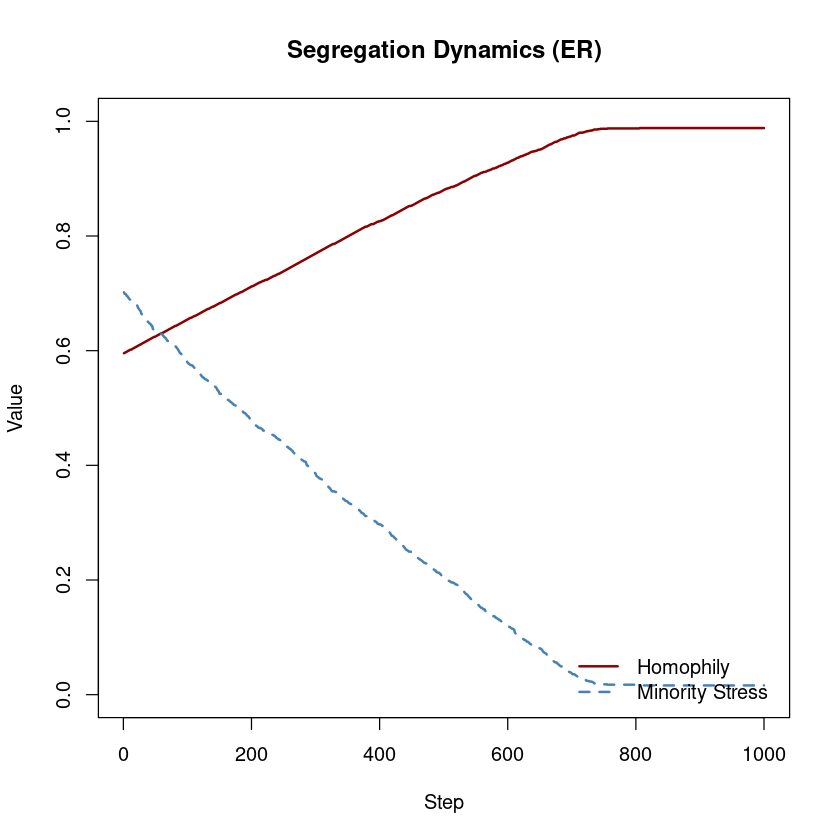
\includegraphics[width=\linewidth]{images/henryer.png}
        \caption{Erdős–Rényi}
        \label{fig:henryer}
    \end{minipage}
    \hfill
    \begin{minipage}[t]{0.24\linewidth}
        \centering
        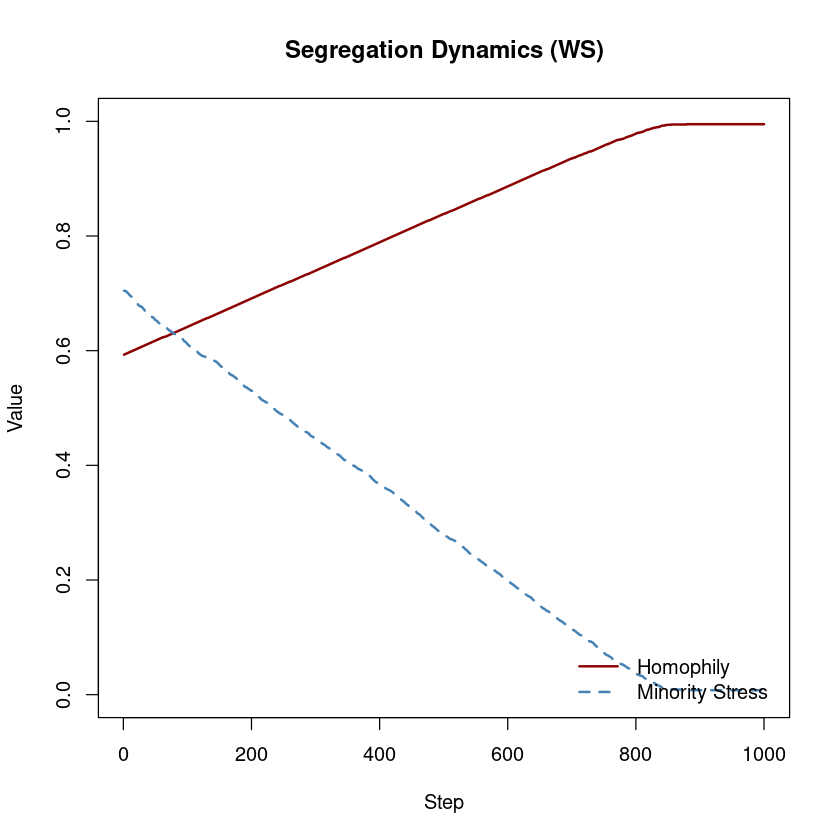
\includegraphics[width=\linewidth]{images/henryws.png}
        \caption{Watts–Strogatz}
        \label{fig:henryws}
    \end{minipage}
    \hfill
    \begin{minipage}[t]{0.24\linewidth}
        \centering
        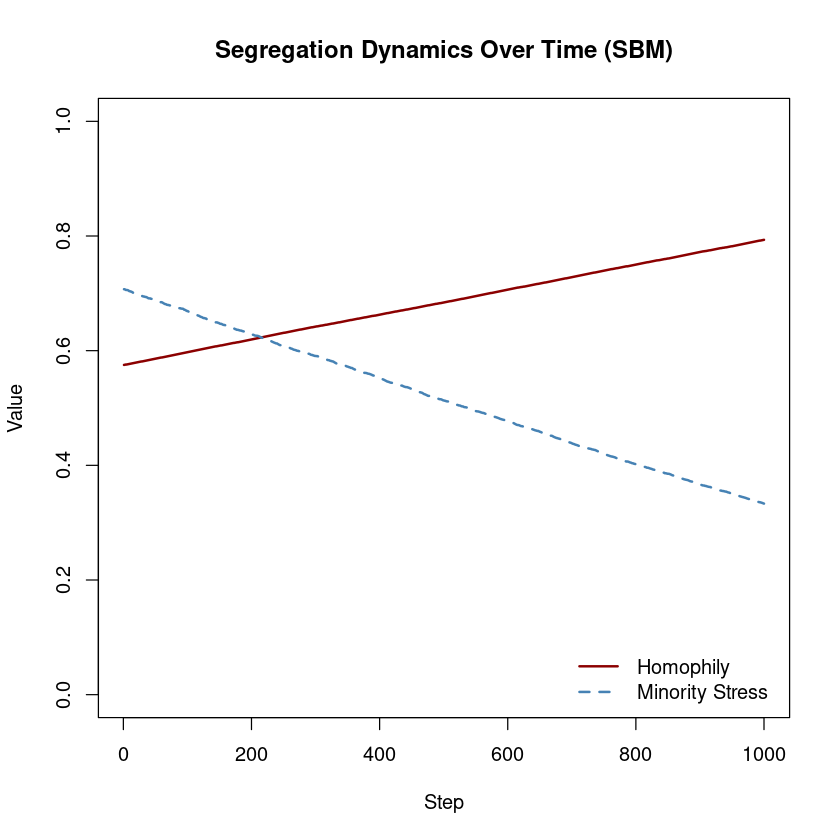
\includegraphics[width=\linewidth]{images/henry2.png}
        \caption{Stochastic Block Model}
        \label{fig:henrysbm}
    \end{minipage}
    \caption{Comparison of network models under the Henry framework.}
    \label{fig:henry_four}
\end{figure}

\newpage